%\documentclass[10pt,onecolumn,a4paper]{article}
\documentclass{article} % For LaTeX2e
\usepackage{times}
\usepackage{url}
\usepackage{epsfig}
\usepackage{graphicx}

\usepackage{algorithm, algorithmic}
\usepackage{amsmath, amsthm, amssymb}

\usepackage{natbib}
\usepackage{bibentry}
\usepackage{hyperref}
\usepackage[nolist]{acronym}
\usepackage{fullpage}

\renewcommand{\Pr}{\field{P}}

\newcommand{\bx}{\boldsymbol{x}}
\newcommand{\bX}{\boldsymbol{X}}
\newcommand{\bu}{\boldsymbol{u}}
%\newcommand{\bu}{h}
\newcommand{\h}{h}
\newcommand{\by}{\boldsymbol{y}}
\newcommand{\bY}{\boldsymbol{Y}}
\newcommand{\bH}{\boldsymbol{H}}
\newcommand{\sY}{\mathcal{Y}}
\newcommand{\bhatY}{\boldsymbol{\hat{Y}}}
\newcommand{\bbary}{\boldsymbol{\bar{y}}}
\newcommand{\bg}{\boldsymbol{g}}
\newcommand{\bz}{\boldsymbol{z}}
%\newcommand{\bzt}{k(\bx_t,\cdot)}
\newcommand{\bzt}{k_t}
\newcommand{\bzi}{k_i}
\newcommand{\bZ}{\boldsymbol{Z}}
\newcommand{\bbarZ}{\boldsymbol{\bar{Z}}}
\newcommand{\bbarz}{\boldsymbol{\bar{z}}}
\newcommand{\bhatZ}{\boldsymbol{\hat{Z}}}
\newcommand{\bhatz}{\boldsymbol{\hat{z}}}
\newcommand{\bbarw}{\bar{f}}
\newcommand{\barz}{\bar{z}}
\newcommand{\bS}{\boldsymbol{S}}
\newcommand{\bbarS}{\boldsymbol{\bar{S}}}
\newcommand{\bw}{\boldsymbol{w}}
%\newcommand{\bw}{f}
\newcommand{\f}{f}
\newcommand{\bW}{\boldsymbol{W}}
\newcommand{\bU}{\boldsymbol{U}}
\newcommand{\bv}{\boldsymbol{v}}
\newcommand{\bzero}{\boldsymbol{0}}
\newcommand{\balpha}{\boldsymbol{\alpha}}
\newcommand{\sA}{\mathcal{A}}
\newcommand{\sC}{\mathcal{C}}
\newcommand{\sX}{\mathcal{X}}
\newcommand{\sS}{\mathcal{S}}
\newcommand{\sZ}{\mathcal{Z}}
\newcommand{\sbarZ}{\bar{\mathcal{Z}}}
\newcommand{\fbag}{\bold{F}}


\newcommand{\inner}[1]{ \langle {#1} \rangle }

%\newcommand{\argmin}[1]{\underset{#1}{\operatorname{argmin}}}
\DeclareMathOperator*{\argmin}{arg\,min}
\DeclareMathOperator*{\argmax}{arg\,max}
%\newcommand{\argmax}[1]{\underset{#1}{\operatorname{argmax}}}

\newcommand{\todo}[1]{\textcolor{red}{TODO: #1}}
\newcommand{\fixme}[1]{\textcolor{red}{FIXME: #1}}

\newcommand{\field}[1]{\mathbb{#1}}
\newcommand{\set}[1]{\mathcal{#1}}
\newcommand{\fY}{\set{Y}}
\newcommand{\fX}{\set{X}}
\newcommand{\fH}{\set{H}}

\newcommand{\R}{\field{R}}
\newcommand{\Nat}{\field{N}}
\newcommand{\E}{\field{E}}
\newcommand{\Var}{\mathrm{Var}}

\newcommand{\X}{\mathcal{X}}
\newcommand{\Y}{\mathcal{Y}}


\newcommand{\btheta}{{\boldsymbol{\theta}}}
%\newcommand{\btheta}{g}
\newcommand{\bbartheta}{\boldsymbol{\bar{\theta}}}
\newcommand\theset[2]{ \left\{ {#1} \,:\, {#2} \right\} }
\newcommand\inn[2]{ \left\langle {#1} \,,\, {#2} \right\rangle }
\newcommand\innK[2]{ \left\langle {#1} \,,\, {#2} \right\rangle_K }
\newcommand\RE[2]{ D\left({#1} \| {#2}\right) }
\newcommand\Ind[1]{ \left\{{#1}\right\} }
\newcommand{\norm}[1]{\left\|{#1}\right\|}
\newcommand{\diag}[1]{\mbox{\rm diag}\!\left\{{#1}\right\}}

\newcommand{\defeq}{\stackrel{\rm def}{=}}
\newcommand{\sgn}{\mbox{\sc sgn}}
\newcommand{\scI}{\mathcal{I}}
\newcommand{\scO}{\mathcal{O}}

\newcommand{\dt}{\displaystyle}
\renewcommand{\ss}{\subseteq}
\newcommand{\wh}{\widehat}
\newcommand{\ve}{\varepsilon}
\newcommand{\hlambda}{\wh{\lambda}}
\newcommand{\yhat}{\wh{y}}

\newcommand{\hDelta}{\wh{\Delta}}
\newcommand{\hdelta}{\wh{\delta}}
\newcommand{\spin}{\{-1,+1\}}

\newcommand{\theHalgorithm}{\arabic{algorithm}}

\newtheorem{lemma}{Lemma}
\newtheorem{theorem}{Theorem}
\newtheorem{cor}{Corollary}
\newtheorem{definition}{Definition}
\newtheorem{assumption}{Assumption}
%\newtheorem{remark}{Remark}
%\newtheorem{prop}{Proposition}

\newcommand{\reals}{\mathbb{R}}
\newcommand{\sign}{{\rm sign}}


\newcommand{\q}{q}
\renewcommand{\ng}{\theta}

\newcommand{\G}{\mathcal{G}}
\newcommand{\W}{\mathcal{W}}
\newcommand{\opteps}{\eps^*}

\newcommand{\Risk}{\mathcal{R}}
\newcommand{\RiskLoss}{\mathcal{E}^{\ell}}
\newcommand{\Ltworho}{\mathcal{L}^2_{\rho_\fX}}
\newcommand{\Lonerho}{\mathcal{L}^1_{\rho_\fX}}
\newcommand{\frho}{f_\rho}
\newcommand{\flrho}{f^{\ell}_\rho}
\newcommand{\fcla}{f_c}
\newcommand{\fl}{f^{\ell}}
\newcommand{\flambda}{f_\lambda}
\newcommand{\HK}{\mathcal{H}_K}

%\newcommand{\normK}[1]{\left\|{#1}\right\|_{\mathcal{H}_K}}
\newcommand{\normK}[1]{\left\|{#1}\right\|_K}
\newcommand{\normL}[1]{\left\|{#1}\right\|_{\Ltworho}}
\newcommand{\normLOne}[1]{\left\|{#1}\right\|_{\Lonerho}}

\DeclareMathOperator\erf{erf}

\newcommand{\gain}{Reward}
\newcommand{\sg}{G}

\begin{acronym}
\acro{EG}{Exponentiated Gradient}
\acro{DFEG}{Dimension-Free Exponentiated Gradient}
\acro{OMD}{Online Mirror Descent}
\acro{ASGD}{Averaged Stochastic Gradient Descent}
\acro{SGD}{Stochastic Gradient Descent}
\acro{PiSTOL}{Parameter-free STOchastic Learning}
\acro{OCO}{Online Convex Optimization}
\acro{OLO}{Online Linear Optimization}
\acro{RKHS}{Reproducing Kernel Hilbert Space}
\acro{IID}{Independent and Identically Distributed}
\acro{SVM}{Support Vector Machine}
\acro{ERM}{Empirical Risk Minimization}
\acro{COCOB}{Continous Coin Betting}
\end{acronym}

\newcommand{\ignore}[1]{}
\newcommand{\nobibentry}[1]{{\let\nocite\ignore\bibentry{#1}}}

\begin{document}
\nobibliography*

%%%%%%%%% TITLE
\title{Betting against a Continuos Coin}
\author{
\begin{tabular}{c@{\hskip 1in}c}
  Francesco Orabona & David Pal \\
  francesco@orabona.com & dpal@yahoo-inc.com \\
\end{tabular}
\\\\
Yahoo Labs \\
New York, NY, USA
}


\maketitle



\begin{abstract}%   <- trailing '%' for backward compatibility of .sty file
Bla
\end{abstract}

\section{Introduction}
\label{sec:intro}

\acresetall

\ac{OCO} is a problem where an algorithm repeatedly chooses a point $\bw_t$ from a convex decision set $K$, observes an arbitrary, or even adversarially chosen, loss function $\bg_t$ and suffers loss $f_t(\bw_t)$, where $f_t$ is a convex function.  The goal of the algorithm is to have a small cumulative loss. Performance of an algorithm is evaluated by the so-called regret, which is the difference of cumulative losses of the algorithm and of the (hypothetical) strategy that would choose in every round the same best point in hindsight.
Typically, one tries to prove that the regret grows at most sub-linearly in time, that is, the average regret vanishes over time.

Typically, \ac{OCO} is solved with a reduction of a \ac{OLO} problem~\citep{Cesa-BianchiL06,Shalev-Shwartz12}, where the losses $f_t(bw)$ are the linear functions $\langle \bw, \bg_t\rangle$.
Indeed, many learning problems can be directly phrased as \ac{OLO}, e.g., learning with expert advice~\citep{LittlestoneW94,Vovk98,Cesa-BianchiFHHSW97}, online combinatorial optimization~\cite{KoolenWK10}. A part from \ac{OCO}, other problems can be also reduced to \ac{OLO}, e.g. online classification and regression~\citep[Chapters~11~and~12]{Cesa-BianchiL06}, multi-armed problems~\citep[Chapter~6]{Cesa-BianchiL06}, and batch and stochastic optimization of convex functions~\cite{NemirovskyY83}.  Hence, a result in \ac{OLO} immediately implies other results in all these domains.

However, as essential as it is, being able to solve an optimization problem is only half of the problem in machine learning. In fact, we are often interested in the generalization performance of a predictor trained from data. This depends not only on the ability to optimize a loss but also on constraining the complexity of the predictor. This is usually achieved through the use an regularized objective function, that biases the solution towards a small region of the space. However, choosing the size of this region is usually a problem by itself, that is solved by practitioners with a variety of more or less theoretical principled tools.

In this paper, we claim that a more fundamental notion subsumes both \ac{OLO} and \ac{OCO}. This notion is linked to the ability of an algorithm to optimally bet on an arbitrary sequence of outcomes from a coin. We will define the notion of \ac{MBA} that not only will allow us to solve \ac{OLO} and \ac{OCO}, but to design algorithm that do not require any explicit form of regularization nor any hyper-parameter to tune, yet are able to achieve optimal worst case guarantees. 
In particular, we will show that an algorithm that guarantees a reward close to the optimal sequence of bets also guarantees optimal regret in \ac{OLO}/\ac{OCO} and automatic model selection in regularized \ac{ERM}.

We will also show connections between the optimal the betting strategy known in economics as Kelly betting \citep{Kelly56} and online learning, and hence indirectly with stochastic optimization and statistical learning.
\section{Setting and Notation}
These papers deals with three different settings, hence we will fist describe the common notation and then each of one them separately, trying to show the similarities between them.

Real number variable will denoted by italic letters, e.g. $x,y$, while vectors will be denoted by bold letters, $\bw,\bu$.
We define the KL divergence between two Bernoulli distributions with parameters $p$ and $q$ as
\[
D(p||q) := p \log\frac{p}{q} + (1-p) \log\frac{1-p}{1-q}.
\]
Hence, we have, for any $ 0\leq p < 1$
\[
D\left(\frac{1}{2}+\frac{p}{2}\middle\|\frac{1}{2}\right) = D\left(\frac{1}{2}-\frac{p}{2}\middle\|\frac{1}{2}\right)= \frac{1+p}{2} \log(1+p) + \frac{1-p}{2} \log(1-p).
\]
The extension for continuity of $D(\frac{1}{2}+\frac{p}{2}||\frac{1}{2})$ in $p=1$ is $\log(2)$.
Also,
\[
\left(\frac{n}{n-q}\right)^{n-q} \left(\frac{n}{q}\right)^{q} = 2^n \exp\left(-n D\left(\frac{q}{n}\middle\|\frac{1}{2}\right)\right),
\]
and
\[
\left(1+x\right)^\frac{1+x}{2} \left(1-x\right)^\frac{1-x}{2}= \exp\left( D\left(\frac{1}{2}+\frac{x}{2}\middle\|\frac{1}{2}\right) \right)
\]

\textbf{Binary and Continuos Coin Betting.}
The bettor starts with the amount of money $\epsilon$. 
At the end of each bet in the time step $t$ we denote the amount of money he has by $\gain_t$.
At each time step $t$, it has to bet a quantity of money $w_t$ equal to a fraction of his current money, $w_t:=\beta_t \, \gain_{t-1}$ where $\beta_t \in (-1,1)$. Note that here we consider only betting strategies that will never result in a negative quantity of money owned. Hence, $|\beta_t|$ must be strictly less than 1, otherwise the algorithm could lose all the money in one round.
After the bet, the outcome of the coin $g_t \in \{-1,1\}$ is revealed and the better wins (or loses) the quantity $w_t g_t$.
Note that we will speak about a ``binary coin'' when the outcome of the coin is in $\{-1,1\}$, and ``continous coin'' when $g_t \in [-1,1]$. The latter case model the situation in there are different possible prizes with unknown probabilities to be won. Given the quantities above we have $\gain_t:=\gain_{t-1} + w_t g_t = \epsilon + \sum_{i=1}^t w_i g_i$, so that $\gain_0=\epsilon$.

\textbf{\ac{OLO} and \ac{OCO}.}
In the \ac{OLO} framework, at each round $t$ the algorithm receives a vector $\bx_t \in \fX$, picks a $\bw_t \in \fX$, and pays $-\langle \bw_t,\bx_t \rangle$.
The aim of the algorithm is to minimize the \emph{regret}, that is the difference between the cumulative loss of the algorithm, $-\sum_{t=1}^n \langle \bw_t,\bx_t \rangle$, and the cumulative loss of an arbitrary and fixed competitor $\bu \in \fX$, $-\sum_{t=1}^n \langle \bu,\bx_t \rangle$.
In particular, define
\[
Regret_n(\bu) := \sum_{t=1}^n \langle \bg_t , \bu - \bw_t \rangle~.
\]
A vector $\bx$ is a subgradient of a convex function $\ell$ at $\bv$ if $\ell(\bu) - \ell(\bv) \ge \langle \bu - \bv, \bx \rangle$ for any $\bu$ in the domain of $\ell$. The differential set of $\ell$ at $\bv$, denoted by $\partial \ell(\bv)$, is the set of all the subgradients of $\ell$ at $\bv$.

\textbf{Regularized ERM.}
Let $\rho$ a fixed but unknown distribution on $\fX \times \fY$, where $\fY=[-1,1]$.
Denote by $\frho(x):= \int_\fY y d\rho(y|x)$ the \emph{regression function}, where $\rho(\cdot|x)$ is the conditional probability measure at $x$ induced by $\rho$. 
%Denote by $\rho_\fX$ the marginal probability measure on $\fX$ and let $\Ltworho$ be the space of square integrable functions with respect to $\rho_\fX$, whose norm is denoted by $\normL{\f}:=\sqrt{\int_\fX \f^2(x) d \rho_\fX}$. Note that $\frho \in \Ltworho$.
Performance is measured w.r.t. a loss function $\ell: \R \times \R \rightarrow \R_+$, convex and \emph{$L$-Lipschitz} w.r.t. the first argument.% We will consider \emph{$L$-Lipschitz} losses, that is $|\ell(x)-\ell(x')| \leq L |x-x'|$.
Define the \emph{$\ell$-risk} of $f$, as $\RiskLoss(f):=\int_{\fX \times \fY} \ell(y f(x)) d \rho$. Also, define $\flrho(x):=\argmin_{t \in \R} \int_\fY \ell(y t) d \rho(y|x)$, that gives the \emph{optimal $\ell$-risk}, $\RiskLoss(\flrho)=\inf_{\f \in \Ltworho} \RiskLoss(\f)$.
%, \ \forall x,x' \in \R$, and \emph{$H$-smooth} losses, that is differentiable losses with the first derivative $H$-Lipschitz. Note that a loss can be both Lipschitz and smooth.
Given a training set $\{\bx_t,y_t\}_{t=1}^n$ of samples drawn \ac{IID} from $\rho$, the regularized \ac{ERM} strategy finds a predictor $\hat{f}$ in a functional space $\fH$, such that
\[
\hat{f}= \argmin_f \lambda R(f) + \frac{1}{n} \sum_{t=1}^n \ell(f(\bx_t),y_t),
\]
where $R(f)$ is the regularizer.
\section{Betting, OLO, OCO, Stochastic Optimization, and Model Selection}
\label{sec:appl}

\begin{figure}[t]
\centering
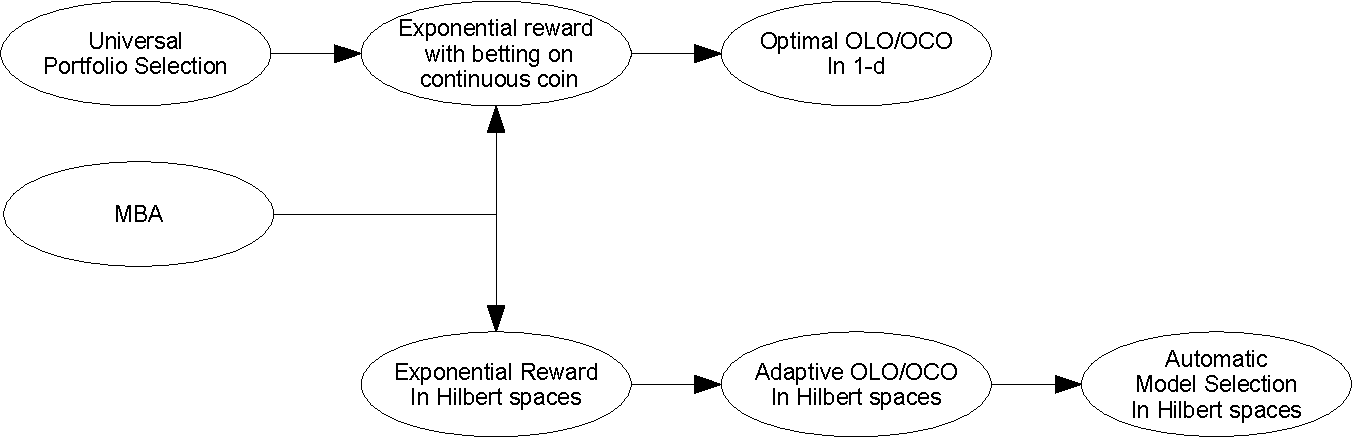
\includegraphics[width=.95\linewidth]{./figs/links_between_areas.pdf}
\caption{The links between the different areas and betting.}
\end{figure}

In this section we will show the connection between portfolio selection, betting on a continous coin, adaptive \ac{OLO}/\ac{OCO}, and automatic model selection. We will prove that, given an ``optimal'' betting algorithm, the same algorithm can be used to solve all the problems listed above.

We will assume that a 1-dimensional algorithm exists, that satisfies the following assumption.
\begin{assumption}
\label{assumption:1-d_algo}
Assume that there exists a sequence of functions $f:\R \times Set \rightarrow \R$ convex in the first argument and an algorithm, that we will denote by \ac{MBA}, that generates $b_t$, where $|b_t|\leq 1$, using in input $x_{t-1} \in \R$, $z_1, \ldots, z_{t-1} \in [-1,1]$, such that the following holds
\begin{equation}
\label{eq:1_d_hp}
(1+b_t z_t) f\left( x_{t-1}^2, \{|z_1|, \ldots, |z_{t-1}|\} \right) \geq f\left( (x_{t-1}+z_t)^2, \{|z_1|, \ldots, |z_t|\}\right), \ \ \forall z_{t} \in [-1,1]~.
\end{equation}
\end{assumption}

By induction is easy to prove that such algorithm can indeed be used as a betting algorithm. 
\begin{theorem}
\label{theo:1-d_reward}
Assume that Assumption \ref{assumption:1-d_algo} holds and use the \ac{MBA} with $x_{t-1}=|\sum_{i=1}^{t-1} g_i|$ and $z_t=g_t$.
Then, for any sequence of outcomes $g_t \in [-1,1]$, the following holds
\[
\gain_n \geq f\left( \left(\sum_{i=1}^{t-1} g_i \right)^2, \left\{|z_1|, \ldots, |z_n|\right\}\right)~.
\]
\end{theorem}

Even more importantly, the \ac{MBA} can also be used to prove lower bound on the reward in Hilbert Spaces.
%\noindent\textbf{From 1-dimension to Hilbert spaces.}
\begin{theorem}
\label{theo:hilbert_reward}
  Assume that \ref{assumption:1-d_algo} holds.
  Let $\bg_t \in \fH$ an arbitrary sequence of vector, such that $\norm{\bg_t} \leq 1$ and define the vector $\btheta_t=\sum_{i=1}^{t} \bg_i$.
  Use the Algorithm in \ref{assumption:1-d_algo} with the sequence $x_{t-1}= \norm{\btheta_{t-1}}$.
  Define a vectorial algorithm that at each step outputs $\bw_t = b_t \frac{\btheta_{t-1}}{\norm{\btheta_{t-1}}} \gain_{t-1}$. Then the following holds
  \[
  \sum_{t=1}^n \langle \bg_t, \bw_t \rangle \geq f_n\left( \norm{\sum_{t=1}^n \bg_t}^2, \left\{\norm{\bg_1}, \ldots, \norm{\bg_n}\right\}\right)~.
  \]
\end{theorem}
This theorem is useful to prove regret bounds in Hilbert spaces, as shown in the next part.

\vspace{0.2cm}\noindent\textbf{From Reward to Regret.}
The reward and regret view on online learning are equivalent: an algorithm guarantees low regret iff it guarantees high reward. The following Theorem makes this claim rigorous. Notice that the algorithm is exactly the same in the two setting.
\begin{theorem}[\citet{McMahanO14}]
  \label{thm:rrdual}
  Let $\Psi:\mathcal{H} \rightarrow (-\infty, +\infty]$ be a lower semicontinuos and convex function, with $dom \Psi \neq \emptyset$. An
  algorithm for the player guarantees
  \[
  \gain_n \geq \Psi\left(\sum_{t=1}^n \bg_t\right) - \epsilon \quad \quad \quad \textnormal{ for any } \bg_1, \dots, \bg_n
  \]
  for a constant $\epsilon \in \R$ if and only if it
  guarantees
  \begin{equation}\label{eq:regb}
  \qquad Regret_n(\bu) \leq \Psi^*(\bu) + \epsilon \quad \quad \quad \textnormal{ for all } \bu \in \mathcal{H}~.
  \end{equation}
\end{theorem}
So, a betting algorithm can be used for online learning and vice-versa. However, as it was already stressed in \citet{McMahanO14}, the reward view has the big advantage of having one variable less, the competitor $\bu$.
Moreover, as we will show in Section~\ref{sec:algo}, designing and analysing algorithms in one of the two views could be much easier than in the other one.
Coupling Theorem~\ref{thm:rrdual} with Theorem~\ref{theo:hilbert_reward}, we have the following Corollary.
\begin{cor}
\label{theo:hilbert_regret}
Assume that \ref{assumption:1-d_algo} holds. Then there exists a reduction of the \ac{MBA} that produces a sequence of vectors $\bw_t$ that satisfy
\[
Regret_n(\bu) \leq f^*\left( \norm{\sum_{i=1}^{t-1} \bg_i}^2, \left\{\norm{\bg_1}, \ldots, \norm{\bg_n}\right\}\right),
\]
where the conjugation is taken w.r.t. the first argument of $f$.
\end{cor}

\vspace{0.2cm}\noindent\textbf{\ac{OLO}, \ac{OCO} and Stochastic Convex Optimization.}
From the property of the sub-gradient of a convex function we have that, for any sequence of convex functions $f_1, \ldots, f_n$, vectors $\bw_1,\ldots, \bw_n$, and $\bg_t \in f_t(\bw_t)$, we have
\[
Regret^{OCO}_n(\bu) = \sum_{t=1}^n \left( f_t(\bw_t) -f_t(\bu)\right) \leq \sum_{t=1}^n \langle \bw_t-\bu, \bg_t\rangle = Regret_n(\bu)~.
\]
Hence, the regret w.r.t. to arbitrary convex functions is upper bounded by linear regret. This means that an \ac{OLO} algorithm can be used to solve an \ac{OCO} problem, just feeding the algorithm with loss vectors $g_t$ equal to the subgradients of the functions $f_t$.

Also, a regret bound can be transformed into a convergence guarantee for optimization of convex functions.
In particular, we have the following Theorem from~\citet{Cesa-BianchiCG04}.
%
\begin{theorem}
\label{theo:online_to_batch}
Let $\bw_1, \cdots, \bw_n \in \fH$ the vector produced by an OLO algorithm with a regret guarantee $Regret_n(\bu)$.
Let $F:\fH\rightarrow\R$ a convex function, and fix the vectors $\bg_t$ to be unbiased estimate of the gradient of $F$ in $\bw_t$. Then, the following holds
\[
\E\left[F\left(\frac{1}{n} \bw_t\right)\right] \leq \frac{\E[Regret_n(\bu)]}{n}~.
\]
\end{theorem}

High probability bounds can be also easily obtained, assuming more on the function $F$~\citep{Cesa-BianchiCG04}.
The above theorem says that, if the regret grows, for example, as $\scO(\sqrt{n})$, the OLO algorithm can be used as a stochastic optimization algorithm with convergence in expectation $\scO(\frac{1}{\sqrt{n}})$.


\vspace{0.2cm}\noindent\textbf{Adaptive Algorithms for OLO and Self-tuning Model Selection.}
In learning theory a key concept is the one of regularization. If the concept class we are learning is too rich, we need to constrain the complexity of the trained predictor. A regularizer is achieving this, biasing the classifieres towards a small region of the space. However, it is known that the optimal amount of regularization is completely problem-dependent. Hence, the regularizer becomes another parameter to be learned.

Most, if not all, the machine learning algorithms uses a two-stages process to find the optimal amount of regularization. First, the algorithm is trained with a fixed regularization parameter. Second, its generalization performance is estimated together with a change in the regularization parameter. These two steps are repeated till convergence.

Surprisingly enough, \citep{Orabona14} proved that, when the regularizer is the squared norm of the Hilbert space, the above lenghty procedure can be avoided with a stochastic learner.
In particular, instead of solving a series of regularized ERM problems, with different amounts of regularization, one can use a simple prarameter-free stochastic gradient descent procedure over the training samples and achieve the same performance.
More rigorously, the follwing theorem holds.
\begin{theorem}
\label{theo:self_tune}
Assume that there is an online algorithm whose $Regret_n(\bu)$ is $\scO\left(\norm{\bu}\sqrt{n \ln(n)}\right)$. Then the following holds
\begin{equation}
\label{eq:self_tune}
\E\left[\RiskLoss\left(\frac{1}{T} \sum_{t=1}^n \bw_t\right)\right] \leq \tilde{\scO}\left(\inf_{\bu} \min_{\lambda>0} \RiskLoss(\bu) + \lambda \norm{\bu}^2 +\frac{1}{n \, \lambda} \right)~.
\end{equation}
% Let $\bw_1, \cdots, \bw_n \in \fH$ the vector produced by the PiSTOL algorithm.
% Let $\ell:\R\rightarrow\R$ a convex and Lipschitz function, and fix the vectors $\bg_t$ to be unbiased estimate of the gradient of $F$ in $\bw_t$. Then, the rate of convergence of $\E\left[Risk_F\left(\frac{1}{n} \bw_t\right)\right]$ is the same of regularized ERM algorithm with the (unknown) optimal amount of regularization.
\end{theorem}
To better appreciate this bound, it is useful to compare it with a generalization bound you get from a regularized \ac{ERM} solution, e.g. the one in \citet{SridharanSSS09}.
There, they prove that, with probability at least $1-\delta$, we have
\begin{equation}
\label{eq:fast_rate_srebro}
\RiskLoss\left(\hat{\bw}\right) \leq \tilde{\scO}\left(\inf_{\bu} \RiskLoss(\bu) + \lambda \norm{\bu}^2 +\frac{\ln \frac{1}{\delta}}{\lambda \, n} \right),
\end{equation}
where 
\begin{align*}
\hat{\bw}=\argmin_{\bw} \frac{\lambda}{2}\norm{\bw}^2 + \sum_{t=1}^n f_t(\bw_t)~.
\end{align*}
Ignoring the fact that the bound in Theorem~\ref{theo:self_tune} is only in expectation, the bound in \eqref{eq:fast_rate_srebro} is missing the minimum over $\lambda$, that is present in \eqref{eq:self_tune}. Hence, to obtain the optimal performance in the regularized \ac{ERM} setting we have to prove different values of $\lambda$, while in Theorem~\ref{theo:self_tune} the tuning is automatic. This is particular important in infinite dimensional Hilbert spaces, where the infimum could not be attained by a vector in the space~\cite{Orabona14}.

The only missing piece is to prove that the existence of the \ac{MBA} guarantees to have an algorithm that satisfies the regret guarantee in the hypothesis of Theorem~\ref{theo:self_tune}. Indeed, we have the following Theorem.
\begin{theorem}
\label{theo:regret_pistol}
Assume that \ref{assumption:1-d_algo} holds and that the function $f$ is exponential in his first argument.
Then there exists an algorithm, that uses the \ac{MBA} as a subroutine, that guarantees $Regret_n(\bu)=\scO\left(\norm{\bu}\sqrt{n \ln(n)}\right)$.
\end{theorem}

%In reality, the connection between betting and self-tuning regularized ERM is actually stronger. In fact, the following theorem can be proved.
%\begin{theorem}
%If a betting strategy against a coin with outcomes in $[-1,1]$ guarantees an exponential reward, the same algorith used for SGD over the risk of a convex loss will guarantee optimal rate of convergence to the Bayes risk.
%\end{theorem}


To summarize, the existence of a simple 1-d algorithm guarantees, though a straighforward reduction, the possibility of learning in Hilbert spaces, in the online setting and stochastic setting, with optimal rates.
In the next section we will explain what are the difficulties in designing such 1-d algorithm and in Section~\ref{sec:algo} we will present our solution.
\section{Kelly Betting, Mixture Forecasters and Portfolio Selection}
\label{sec:kelly}

Before trying to design the \ac{MBA}, we will explore what are the theoretical limits that such an algorithm should obey. These limits will guide us in the design of the algorithm.

\textbf{Betting on a binary coin.}
Given the link with betting and \ac{MBA}, exploring the limits of the reward obtainable with betting will imply limits on the \ac{MBA}.
We will considere the case that the outcomes are binary, i.e. $g_t \in \{-1,1\}$.
First, we will analyze the class of betting strategy that bets a fixed amount of the current reward for the entire game.
The following theorem is well-known, and it has been shown, for example, in \cite{}.

\begin{theorem}
\label{thm:oracle_fraction}
Let an algorithm bet a fixed fraction of his current reward, i.e. $w_t=\beta \, \wealth_{t-1}$, where $0\leq\beta\leq1$. Then, for any sequence $g_1, \ldots, g_n \in \{-1,1\}$, we have
\begin{equation}
\label{eq:opt_fixed_reward}
\max_{\beta} \ \wealth_{n}
= \epsilon \exp\left(n\, D\left(\frac{1}{2}+\frac{\sum_{t=1}^n g_t}{2 n}\middle\|\frac{1}{2}\right)\right)~. 
%\leq \epsilon \exp\left(\frac{(\sum_{t=1}^T z_t)^2}{2T}+\frac{(\sum_{t=1}^T z_t)^4}{5 T^3}\right).
\end{equation}
Moreover the optimal $\beta$ is $\frac{\sum_{t=1}^n g_t}{n}$.
\end{theorem}

The above theorem tells us that any algorithms that keep the fraction of money to bet at each round fixed cannot gain more that the quantity on the r.h.s. of $\eqref{eq:opt_fixed_reward}$. Moreover, the optimal fraction is nothing else the empirical estimate of the frequencies of 1 vs -1.

One might ask if having a fraction of money that changes over time might help and the answer is substantially negative. The next Theorem shows that we can only hope for logarithmic gain in the exponent w.r.t. \eqref{eq:opt_fixed_reward}.
\begin{theorem}
\label{thm:oracle_fraction_changing}
For $n \in \Nat$ even, any betting strategy $w_t$, and an initial amount of money equal to $\epsilon$, we have
\[
\wealth_{n}
\leq \epsilon \min\left\{\left(\exp\left(\frac{1}{6}\right)\sqrt{2 \pi}\frac{|\sum_{t=1}^n g_t|}{\sqrt{n}} +2\exp\left(\frac{1}{6}\right)-1\right) \exp\left(n\, D\left(\frac{1}{2}+\frac{|\sum_{t=1}^n g_t|}{2 n}\middle\|\frac{1}{2}\right)\right), 2^n\right\}.
\]
\end{theorem}

These last two theorems suggest that we should aim at obtaining an exponential gain, up to logarithmic terms in the exponent.

Notice that, if we knew that the setting is stochastic, the optimal fraction of money in Theorem~\ref{eq:opt_fixed_reward} is nothing else than the Kelly criterion, that is derived with the objective of maximizing the expectation of the logarithm of the reward, rather than the expected profit from each bet~\citep{Kelly56}.
In the latter case, one would be led to gamble all he had when presented with a favorable bet, and, in the case of a lost, one would have no capital with which to place subsequent bets. Kelly realized that it was the logarithm of the gambler's capital which is additive in sequential bets, and "to which the law of large numbers applies."
In most gambling scenarios, the Kelly strategy will do better than any essentially different strategy in the long run \cite{}. The formula has also a practical use [2][3][4].

Practically speaking, the Kelly criterion applied to a coin that has probability $p$ for one of the faces, with $p> \frac{1}{2}$, and with equal wins, corresponds in betting on that face on each round a fraction of the current money equal to $2p-1$. This simple rule assures that in expectation the growth rate will be exponential \textbf{In expectation?}.

However, the Kelly criterion can be used only if the coin is stochastic and if we knew bias of the coin exactly. One might argue that this is equally unlikely as knowning beforehand the empirical frequencies of $1$ and $-1$ in the sequence.
One might ask what is the optimal strategy in the case that the sequence of outcomes of the coin is non-stochastic.
A little known result by Krichevsky and Trofimov~\cite{}, says that above procedure can still be used, substituiting the  unknown probability with a slightly biased running estimate. In particular, the probability of a face at time $t$ is estimated with 
\[
\hat{p_t}=\frac{\text{number of that face in the previous } t-1 \text{ rounds}}{t}.
\]
In particular the following Theorem holds for the Krichevsky and Trofimov algorithm.
\begin{theorem}
Bet at each round a quantity equal to $\hat{p_t} \gain_{t-1}$ on the face that appeared more in the past. Then
\begin{align*}
\gain_{n} 
\geq \epsilon \exp\left(n\, D\left(\frac{1}{2}+\frac{\sum_{t=1}^n z_t}{2 n}\middle\|\frac{1}{2}\right) - \frac{1}{2} \ln n - \ln 2\right)~.
\end{align*}
\end{theorem}

They proved that this simple procedure guarantees an exponential reward as well, only a factor $\sqrt{n}$ less than having known in advance the total number of heads in the sequence of $n$ rounds. It is also known that this factor cannot be improved.

\textbf{Betting on a continuos coin.}
Hence, the problem of betting on a coin is solved. However, the following problem cannot be solved with the Krichevsky-Trofimov forecaster. Consider the same betting scenario as before, with the only difference that the outcome of the coin is now a real number between $+1$ and $-1$. We can interpret this as a betting scenario in which the maximum amount of money that can be won or lost in each bet is fixed, but the actual winnings is shown only after the bet is done. The formalism is still the same, because $w_t g_t$ is still the amount of money won. However, the simple change makes this problem much harder than before. Indeed, to solve it we now have to use a Universal Portfolio algorithm. In fact, it is possible to consider the following equivalent problem. On each time step, we have to divide our wealth between two stocks. The gains given by the market are coded in the vector $m_t$ that are equal to $[1+g_t, 1-g_t]$. The algorithm will return a division of the wealth of the form $[a_t, 1-a_t]$. Then this can be used to bet on the continuos coin using $\beta_t=2 a_t-1$.
It is easy to see that with this reduction the wealth of the portfolio selection is equal to the reward on the continuos coin, that is
\[
\gain_{t-1} \left((1+g_t) a_t+(1-g_t)(1-a_t)\right)=\gain_{t-1}+\gain_{t-1} \beta_t g_t~.
\]
%stocks as $[\frac{1+\beta_t}{2},\frac{1-\beta_t}{2}]$. It is immediate to show that in this way the wealth is multiplied by $1+\beta_t g_t$, as in \eqref{}.

One problem with this reduction is that we cannot have an explicit lower bound on the reward. In fact, the Universal Portfolio algorithm only assures us that the reward is close to the optimal one, but there is no closed formula for the optimal reward.
Also, the Universal Portfolio algorithm strategy itself cannot be computed in a closed formula and it has to be approximated~\cite{KalaiV03}.

\section{COCOB: A Master Betting Algorithm for Continuous Coins}
\label{sec:algo}

\begin{algorithm}[ht]
  \begin{algorithmic}
  {
    \STATE{\bfseries Parameters:} $a>2,\delta>1$
    \STATE{\bfseries Initialize:} $\wealth_0=\epsilon,\sg_0=\delta$
    \FOR{$t=1,2,\dots$}
    \STATE{Receive $\theta_{t-1}$ and $\sg_{t-1}$}
    \STATE{Calculate fraction and direction to bet: $\beta_t=2 \, S\left(\frac{4 \theta_{t-1}}{a (\sg_{t-1} + 1)}\right)-1$}
    \STATE{Bet $b_t=\beta_t \wealth_{t-1}$}
    \STATE{Win (or lose) $b_t z_t$}
    \STATE{Update your money: $\wealth_t=\wealth_{t-1}+b_t z_t$}
    %\STATE{Update $\theta_t$: $\theta_t=\theta_{t-1}+z_t$}
    %\STATE{Update $\sg_t$: $\sg_t=\sg_{t-1}+|z_t|$}
    \ENDFOR
  }
  \end{algorithmic}
  \caption{COCOB}
  \label{alg:cocob}
\end{algorithm}

As said in Section~\ref{sec:appl}, we need an efficient \ac{MBA} algorithm for continuous coin betting.
Hence, in this section we show how a very simple algorithm that satisfies Assumption~\ref{assumption:1-d_algo}.

The first observation is that the wealth of the optimal strategy, as proved in Theorems~\ref{thm:oracle_fraction} and \ref{thm:oracle_fraction_changing}, is expected to grow exponential in time depending on $D\left(\frac{1}{2}+\frac{\sum_{t=1}^n g_t}{2 n}\middle\|\frac{1}{2}\right)$. If we try to achieve exactly this term, we are (probably) doomed to use the universal portfolio selection algorithm or to assume a binary coin.
However, we might try to achieve something that is very close to that quantity.
The idea is to sacrifice a bit of the guaranteed growth of the wealth in order to gain generality. In particular we aim at designing a \ac{MBA}.

It is easy to show that
\[
D\left(\frac{1}{2}+\frac{\sum_{t=1}^n g_t}{2 n}\middle\|\frac{1}{2}\right) \geq \frac{(\sum_{t=1}^n g_t)^2}{2 n^2},
\]
where the approximation is very good around $\sum_{t=1}^n g_t=0$ and it is of the order of $\scO(\frac{(\sum_{t=1}^n g_t)^4}{ n^4})$. It was first proposed (but not solved) by~\cite{McMahanA13} to use the above approximation as a target wealth.
Indeed, we show below that it is possible to design a simple algorithm that has an exponential reward that depends on this quantity. Also, our guarantee will be data-dependent and the resulting algorithm will satisfy Assumption~\ref{assumption:1-d_algo}.

The \ac{COCOB} algorithm is shown in Algorithm~\ref{alg:cocob} and we can prove it is a \ac{MBA}.
%Without loss of generality, we will assume that $g_t$ are between $[-1,1]$.
%
\begin{theorem}
\label{theo:cocob}
Let $a\geq2$. Then the function 
\[
f(x,\{z_1, \ldots, z_t\}) := \epsilon \exp\left(\frac{x^2}{a (1+\delta+\sum_{i=1}^{t-1} z_i)} - \sum_{i=1}^{n} \frac{z_i}{a( 1+\delta+\sum_{j=1}^{i-1} z_j) } \right)
\]
and the betting 
\[
b_t:= \gain_{t-1} \left(2 \, S\left(\frac{4 x}{a (1+\delta+\sum_{i=1}^{t-1} z_i)}\right)-1\right),
\]
satisfy Assumption~\ref{assumption:1-d_algo}.
% 
% and start with an amount of money equal to $\epsilon$. Bet at each round a quantity equal to
% $\gain_{t-1} \left(2 \, S\left(\frac{4 \theta_{t-1}}{a (\sg_{t-1} + 1)}\right)-1\right)$, where $S:\R\rightarrow(0,1)$ and $S(x)=\frac{1}{1+exp(-x)}$ and receive the outcome $g_t \in [-1,1]$. Then
% \begin{align*}
% \gain_{n} 
% \geq \epsilon \exp\left(\frac{\theta_{n}^2}{a \sg_{n}} - \sum_{i=1}^{n} \frac{|g_i|}{a( \sg_{i-1} + 1) } \right)
% \geq \epsilon \exp\left(\frac{\theta_{n}^2}{a \sg_{n}} - \frac{1}{a} \ln \left(\sum_{t=1}^n \frac{|g_i|}{\delta}+1\right) \right)~.
% \end{align*}
\end{theorem}
%
Notice that the $a$ regulates the trade-off between the first and second term. When $a=2$, we maximize the contribute of the first term.

\begin{cor}
Set $a=2$ in Algorithm~\ref{alg:cocob}. Then we have that the following hold

\begin{itemize}
\item Feed Algorithm~\ref{alg:cocob} with $\sg_{t-1}=\sum_{i=1}^{t-1} |g_t| + \delta + 1$ and $\theta_{t-1}=|\sum_{i=1}^{t-1} g_i|$.
Algorithm~\ref{alg:cocob} guarantees an exponential reward in $\frac{(\sum_{t=1}^n g_t)^2}{2 \sum_{t=1}^n |g_t|}$ and a regret w.r.t. any real number $u$ of $\tilde{\scO}(|u| \sqrt{\sum_{t=1}^n |g_t|})$.

\item Feed Algorithm~\ref{alg:cocob} with $\sg_{t-1}=\sum_{i=1}^{t-1} \norm{\bg_t} + \delta + 1$ and $\theta_{t-1}=\norm{\btheta_{t-1}}$.
Predicting with $\bw_t=b_t \frac{\sum_{i=1}^t \bg_t}{\norm{\sum_{i=1}^t \bg_t}}$ guarantees a regret w.r.t. any $\bu \in \fH$ of $\tilde{\scO}(\norm{\bu} \sqrt{\sum_{t=1}^n \norm{\bg_t}})$ and an exponential reward in $\frac{(\sum_{t=1}^n \bg_t)^2}{2 \sum_{t=1}^n \norm{\bg_t}}$.

\end{itemize}
\end{cor}
\section{Lower bound}

Consider now that
\[
L_t=L_{t-1} + u_t \, g_t = L_{t-1} + \beta \, L_{t-1} \, g_t = L_{t-1} (1+\beta \, g_t)
\]
Hence
\[
L_T=\epsilon \prod_{t=1}^T (1+\beta g_t) = \epsilon (1+\beta)^\frac{T+G}{2} (1-\beta)^\frac{T-G}{2}
\]
Setting $\beta=\frac{G}{T}$ we have
\begin{align}
L_T &= \epsilon (1+\frac{G}{T})^\frac{T+G}{2} (1-\frac{G}{T})^\frac{T-G}{2} 
&= \epsilon \left[(1+\frac{G}{T})^\frac{1+\frac{G}{T}}{2} (1-\frac{G}{T})^\frac{1-\frac{G}{T}}{2}\right]^T 
&\leq \epsilon \exp \left(\frac{G^2}{2 T} + \frac{G^4}{5 T^3}\right)
\end{align}
where we used the fact that
\[
\frac{x^2}{2} +\frac{x^4}{12}\leq \frac{1+x}{2} \log(1+x) + \frac{1-x}{2}\log(1-x) \leq \frac{x^2}{2} + \frac{x^4}{5}
\]
or 
\[
\frac{x^2}{2} +\frac{x^4}{12}\leq \frac{1+x}{2} \log(1+x) + \frac{1-x}{2}\log(1-x) \leq \frac{x^2}{2} + \log(2)-.5
\]
where the lhs is given by Taylor expansion.



\begin{theorem}
Let the sequence of losses be composed by linear losses in $[-1,1]$. For any sequence of predictions $w_t$ and 
for any distribution $B$ on $[-1,1]$ with mean 0, we have 
\[
\max_u \max_{g_1, \ldots, g_t} \sum_{t=1}^T (w_t-u) g_t - f(u) \geq \E_{g_1, \cdots, g_T \sim B} \left[f^*(-\sum_{t=1}^T g_t)\right]
\]
\end{theorem}
\begin{proof}
We have
\begin{align}
\max_u \max_{g_1,\ldots,g_T} &\sum_{t=1}^T (w_t - u) \, g_t -f(u)\\
&\geq \max_u \E_{g_1,\ldots,g_T} [\sum_{t=1}^T (w_t - u) \, g_t -f(u)]\\
&\geq \max_u \E_{g_1,\ldots,g_T} [-\sum_{t=1}^T u \, g_t -f(u)].
\end{align}
We now set $u=\nabla f^*(-\sum_{t=1}^T g_t)$ and use the equality $f(\nabla f^*(p) ) + f^*(p) = p\, \nabla f^*(p)$
\[
\E_{g_1,\ldots,g_T} [-\sum_{t=1}^T u \, g_t -f(u)] = \E_{g_1,\ldots,g_T} \left[f^*(-\sum_{t=1}^T g_t)\right].
\]
\end{proof}

\begin{cor}
Let the sequence of losses be composed by linear losses in $[-1,1]$.
For any distribution $B$ on $[-1,1]$ with mean 0, we have 
\[
\max_u \max_{g_1, \ldots, g_t} \sum_{t=1}^T (w_t-u) g_t - f^*(u) 
\geq \epsilon \exp\left(\frac{T}{\alpha}\right) 2^{-T} \left(1+\exp(\frac{-4}{\alpha})\right)^T.
\]
Also, for $a\geq1.6411$, the lhs decreases in $T$.
\end{cor}
\begin{proof}
Set $f^*(\theta)=\exp\left(\frac{\theta^2}{\alpha T}\right)$.
Choose the distribution on $[-1,1]$, to be $1$ with probability 0.5 and -1 otherwise.
Hence, we have
\begin{align*}
\E_{z\sim B(T,0.5)} \left[\exp\left(\frac{(2 z-T)^2}{\alpha T}\right)\right]
& =\E_{z\sim B(T,0.5)} \left[\exp\left(\frac{T^2 + 4 z^2 - 4 z T }{\alpha T}\right)\right] \\
& =\exp\left(\frac{T}{\alpha}\right) \E_{z\sim B(T,0.5)} \left[\exp\left(\frac{4 z^2 - 4 z T }{\alpha T}\right)\right] \\
& \geq\exp\left(\frac{T}{\alpha}\right) \E_{z\sim B(T,0.5)} \left[\exp\left(\frac{- 4 z T }{\alpha T}\right)\right] \\
& =\exp\left(\frac{T}{\alpha}\right) 2^{-T} \left(1+\exp\left(-\frac{4}{\alpha}\right)\right)^T.
%& \geq \frac{1}{2}\exp\left(\frac{T}{\alpha}\right) \E_{z\sim B(T,0.5)} \left[\left(\exp\left(\frac{2 \sqrt{2} z}{\alpha T}\right)+\exp\left(\frac{- 2 \sqrt{2} z}{\alpha T}\right) \right)\exp\left(\frac{- 4 z }{\alpha}\right)\right]\\
%& = \frac{1}{2}\exp\left(\frac{T}{\alpha}\right) \left(\E_{z\sim B(T,0.5)} \left[\exp\left(\frac{2 \sqrt{2} z-4zT}{\alpha T }\right)\right] +\E_{z\sim B(T,0.5)} \left[ \exp\left(\frac{- 2 \sqrt{2} z-4zT}{\alpha T}\right) \right]\right) \\
%& = \frac{1}{2}\exp\left(\frac{T}{\alpha}\right) 2^{-T} \left(  \left(1+\exp(\frac{2 \sqrt{2}-4T}{\alpha T})\right)^T + \left(1+\exp(\frac{-2 \sqrt{2}-4T}{\alpha T})\right)^T\right) \\
%& \geq \frac{1}{2}\exp\left(\frac{T}{\alpha}\right) 2^{-T} \left(1+\exp(\frac{2 \sqrt{2}-4T}{\alpha T})\right)^T\\
%& \geq \frac{1}{2}\exp\left(\frac{T}{\alpha}\right) 2^{-T} \left(1+\exp(\frac{-4}{\alpha})\right)^T.
\end{align*}
For the second statement, taking the logarithm of last expression we have
\begin{align}
-T\log 2+ \frac{T}{\alpha} + T \log \left(1+\exp\left(-\frac{4}{\alpha}\right)\right),
\end{align}
that numerically has a negative coefficient multiplying T iff $a\geq1.6411$.
\end{proof}

We now state a similar upper bound for the reward
\begin{theorem}
Let $z_t$ in $[-1,1]$. For any sequence of predictions $w_t$ and 
for any distribution $B$ on $[-1,1]$ with mean 0, we have 
\[
\min_{z_1, \ldots, z_t} \sum_{t=1}^T w_t z_t - f(\sum_{t=1}^T z_t) \leq -\E_{g_1, \cdots, g_T \sim B} \left[f(\sum_{t=1}^T g_t)\right]
\]
\end{theorem}

\begin{cor}
Let $z_t$ in $[-1,1]$. For any sequence of predictions $w_t$ we have
\[
\min_{z_1, \ldots, z_t} \sum_{t=1}^T w_t z_t - \epsilon \exp\left(\frac{(\sum_{t=1}^T z_t)^2}{\alpha T}\right) \leq -\epsilon\exp\left(\frac{T}{\alpha}\right) 2^{-T} \left(1+\exp\left(-\frac{4}{\alpha}\right)\right)^T.
\]
%Moreover, for $a\geq 1.64101792\cdots$ we have
%\[
%\min_{z_1, \ldots, z_t} \sum_{t=1}^T w_t z_t - 2\epsilon \exp\left(\frac{\sum_{t=1}^T z_t}{\alpha T}\right) \leq -\epsilon.
%\]
\end{cor}
\appendix
\section{Proofs}
\label{sec:proofs}

First we state some technical lemmas that will be used in the following proofs.

Define the Lambert function $W(x):\R\rightarrow\R$ as the one that satisfies the equality\footnote{For $x<0$ the Lambert function is multivalued. Hence, to avoid complication and because we only need positive arguments, we will define it only for positive values of $x$.}
\begin{equation}
\label{eq:lambert}
x=W(x) \exp \left(W(x)\right), \ \forall x\geq0.
\end{equation}
It satisfies the following properties.
%
\begin{lemma}
The Lambert function satisfies $0.6321 \log(x+1) \leq W(x) \leq \log(x+1), \forall x\geq0$.
\end{lemma}
%
\begin{proof}
We first prove the lower bound. From \eqref{eq:lambert} we have
\begin{align}
W(x) &= \log\left(\frac{x}{W(x)}\right) \label{eq:lm_lambert_1} \\
&= \log\left(\frac{x}{\log(x/W(x))}\right). \label{eq:lm_lambert_1b}
\end{align}
From the first equality, for any $a>0$, we get
\[
W(x) \leq \frac{1}{a\, e}\left(\frac{x}{W(x)}\right)^a
\]
that is
\begin{equation}
\label{eq:lm_lambert_2}
W(x) \leq \left(\frac{1}{a\, e}\right)^\frac{1}{1+a} x^\frac{a}{1+a}.
\end{equation}
Using \eqref{eq:lm_lambert_2} in \eqref{eq:lm_lambert_1}, we have
\begin{align*}
W(x) 
\geq \log\left(\frac{x}{\left(\frac{1}{a\, e}\right)^\frac{1}{1+a} x^\frac{a}{1+a}}\right) 
= \frac{1}{1+a}\log\left(a \, e\, x\right)~.
\end{align*}
Consider now the function $g(x)=\frac{x}{x+1} - \frac{b}{\log(1+b) (b+1)} \log(x+1), x\geq b$. This function has a maximum in $x^*=(1+\frac{1}{b}) \log(1+b)-1$, the derivative is positive in $[0,x^*]$ and negative in $[x^*,b]$. Hence the minimum is in $x=0$ and in $x=b$, where it is equal to $0$.
Using the property just proved on $g$, we have that for $x\leq b$, setting $a=\frac{1}{x}$, we have
\begin{align*}
W(x) 
\geq \frac{x}{x+1} \geq \frac{b}{\log(1+b) (b+1)} \log(x+1)~.
\end{align*}
For $x>b$, setting $a=\frac{x+1}{e x}$, we have
\begin{align}
W(x) 
&\geq \frac{e\,x}{(e+1) x + 1} \log(x+1) \geq \frac{e\,b}{(e+1) b + 1} \log(x+1)
\end{align}
Hence, we set $b$ such that 
\[
\frac{e\, b}{(e+1)b + 1} = \frac{b}{\log(1+b) (b+1)}
\]
Numberically, $b=1.71825...$, so
\[
W(x) \geq 0.6321 \log(x+1)~. \qedhere
\]

For the upper bound, we use Theorem~2.3 in \cite{hoorfar2008inequalities}, that says that
\[
W(x) \leq \log\frac{x+C}{1+\log(C)}, \quad \forall x> -\frac{1}{e}, \ C>\frac{1}{e}.
\]
Setting $C=1$, we obtain the stated bound.
\end{proof}

\begin{lemma}
Define $f(\theta)= \beta \exp\frac{x^2}{2 \alpha}$, for $\alpha,\beta>0$, $x\geq0$. Then
\[
f^*(y)=y \sqrt{\alpha W\left(\frac{\alpha y^2}{\beta^2}\right)} - \beta \exp\left(\frac{W\left(\frac{\alpha y^2}{\beta^2}\right)}{2}\right).
\]
Moreover
\[
f^*(y) \leq y \sqrt{\alpha \log \left(\frac{\alpha y^2}{\beta^2} +1 \right)} - \beta.
\]
\end{lemma}
\begin{proof}
From the definition of Fenchel dual, we have
\begin{align*}
f^*(y)= \max_{x} \  x\, y - f(x) = \max_{x} \  x\, y - \beta \exp\frac{x^2}{2 \alpha} \leq x^*\,y -\beta
\end{align*}
where $x^*= \argmax_{x} x\, y - f(x)$. We now use the fact that $x^*$ satisfies $y = f'(x^*)$, to have
\begin{align*}
x^*=\sqrt{\alpha W\left(\frac{\alpha y^2}{\beta^2}\right)},
\end{align*}
where the function $W:\R_+ \rightarrow \R$ is the Lambert function that satisfies
\[
x=W(x) \exp \left(W(x)\right).
\]
Hence, to obtain an upper bound we need an upper bound to the Lambert function.
We use Theorem~2.3 in \cite{hoorfar2008inequalities}, that says that
\[
W(x) \leq \log\frac{x+C}{1+\log(C)}, \quad \forall x> -\frac{1}{e}, \ C>\frac{1}{e}.
\]
Setting $C=1$, we obtain the stated bound.
\end{proof}

\begin{lemma}[ {\citep[Example 13.7]{BauschkeC2011}} ]
Let $\phi:\R \rightarrow (-\infty, +\infty]$ be even. Then $(\phi \ast \norm{\cdot})^*=\phi^* \ast \norm{\cdot}$.
\end{lemma}

\begin{cor}
\label{cor:dual_exp_square}
Define $f(\btheta)= \beta \exp\frac{\norm{\btheta}^2}{2 \alpha}$, for $\alpha,\beta>0$. Then
\[
f^*(y) \leq  \norm{\btheta} \sqrt{\alpha \log \left(\frac{\alpha \norm{\btheta}^2}{\beta^2} +1 \right)} - \beta.
\]
\end{cor}


\subsection{Proof of Theorem~\ref{theo:hilbert_reward}}
\begin{proof}
  For simplicity denote by $f_t(\cdot)=f\left(\cdot, \{\norm{\bg_1}, \ldots, \norm{\bg_t}\}\right)$.
  We will prove the thesis by induction. The base case is verified from the first point of Assumption~\ref{assumption:1-d_algo}. The, we assume that 
  \[
  \epsilon + \sum_{t=1}^{n-1} \langle \bg_t, \bw_t \rangle \geq f_{n-1}\left( \norm{\sum_{t=1}^{n-1} \bg_t}^2\right),
  \]
  and we want to prove that 
  \[
  \epsilon + \sum_{t=1}^{n} \langle \bg_t, \bw_t \rangle \geq f_{n}\left( \norm{\sum_{t=1}^{n} \bg_t}^2\right)~.
  \]
  We have that
  \begin{align*}
  \epsilon + \sum_{t=1}^{n} &\langle \bg_t, \bw_t \rangle - f_n\left( \norm{\sum_{t=1}^{n} \bg_t}^2\right) \\
  &= \langle \bg_n, \bw_n \rangle + \epsilon + \sum_{t=1}^{n-1} \langle \bg_t, \bw_t \rangle - f_n\left( \norm{\sum_{t=1}^{n} \bg_t}^2\right)\\
  &= \left(1+\frac{b_n}{\norm{\btheta_{n-1}}}\langle \btheta_{n-1},\bg_n \rangle \right)\left(\sum_{t=1}^{n-1} \langle \bg_t, \bw_t \rangle +\epsilon \right) - f_n\left( \norm{\sum_{t=1}^{n} \bg_t}^2\right)\\
  &\geq \left(1+\frac{b_n}{\norm{\btheta_{n-1}}}\langle \btheta_{n-1},\bg_n \rangle \right) f_{n-1}\left( \norm{\sum_{t=1}^{n-1} \bg_t}^2\right) - f_n\left( \norm{\sum_{t=1}^{n} \bg_t}^2\right)\\
  &= \left(1+\frac{b_n}{\norm{\btheta_{n-1}}}\langle \btheta_{n-1},\bg_n \rangle \right) f_{n-1}\left( \norm{\btheta_{n-1}}^2\right) - f_n\left( \norm{\btheta_{n-1}}^2 + \norm{\bg_n}^2 + 2 \langle \btheta_{n-1}, \bg_n \rangle \right)\\
  &\geq \min_{r\in \{-1,1\}} \left(1+ r\, b_n \norm{\bg_n} \right) f_{n-1}\left( \norm{\btheta_{n-1}}^2\right) - f_n\left(( \norm{\btheta_{n-1}} + r \norm{\bg_n})^2\right)\\
  &\geq 0,
  \end{align*}
  where the first inequality comes from the induction hypothesis, the second one because we take the minimum of a concave function and the last one by the hypothesis on the \ac{MBA}.
\end{proof}


\subsection{Proof of Theorem~\ref{theo:self_tune}}
\begin{proof}
The statement is readily proved using the inequality $a\,b \leq \frac{a^2}{\lambda} + \lambda b^2, \ \forall a,b\geq0, \lambda>0$ and Theorem~\ref{theo:online_to_batch}.
\end{proof}

\subsection{Proof of Theorem~\ref{theo:regret_pistol}}
\begin{proof}
From Theorem~\ref{theo:hilbert_reward} we have that
\[
\gain_n = \wealth_n - \epsilon  \geq B n^{-C} \exp\left(\frac{\norm{\sum_{t=1}^n \bg_t}^2}{A n}\right)-D - \epsilon~.
\]
We now apply Theorem~\ref{thm:rrdual} and Corollary~\ref{cor:dual_exp_square} to have that 
\[
Regret_n(\bu) \leq \norm{\bu} \sqrt{\frac{A T}{2} \log \left(\frac{\frac{A}{2} T^{2C+1} \norm{\bu}^2}{B^2} +1 \right)} - \frac{B}{T^{C}} + \epsilon+D~. \qedhere
\]
\end{proof}


\subsection{Proofs of Theorem~\ref{thm:oracle_fraction} and Theorem~\ref{thm:oracle_fraction_changing}}

We first state a couple of useful indentities.
For any $ 0\leq p < 1$
\[
D\left(\frac{1}{2}+\frac{p}{2}\middle\|\frac{1}{2}\right) = D\left(\frac{1}{2}-\frac{p}{2}\middle\|\frac{1}{2}\right)= \frac{1+p}{2} \log(1+p) + \frac{1-p}{2} \log(1-p).
\]
The extension for continuity of $D(\frac{1}{2}+\frac{p}{2}||\frac{1}{2})$ in $p=1$ is $\log(2)$.
Also,
\[
\left(\frac{n}{n-q}\right)^{n-q} \left(\frac{n}{q}\right)^{q} = 2^n \exp\left(-n D\left(\frac{q}{n}\middle\|\frac{1}{2}\right)\right),
\]
and
\begin{equation}
\label{eq:div_2}
\left(1+x\right)^\frac{1+x}{2} \left(1-x\right)^\frac{1-x}{2}= \exp\left( D\left(\frac{1}{2}+\frac{x}{2}\middle\|\frac{1}{2}\right) \right)
\end{equation}

Also, for any $-\frac{1}{2} \leq x\leq \frac{1}{2}$ we have
\[
\frac{x^2}{2} +\frac{x^4}{12}\leq D\left(\frac{1}{2}+\frac{x}{2}\middle\|\frac{1}{2}\right) \leq \frac{x^2}{2} + \frac{x^4}{5}.
\]

\begin{proof}[Proof of Theorem~\ref{thm:oracle_fraction}]
From the betting strategy we have
\[
\gain_t=\gain_{t-1} + w_t \, g_t = \gain_{t-1} + \beta \, \gain_{t-1} \, g_t = \gain_{t-1} (1+\beta \, g_t)~.
\]
Hence
\[
\gain_n=\epsilon \prod_{t=1}^n (1+\beta g_t) = \epsilon (1+\beta)^\frac{n+Z}{2} (1-\beta)^\frac{n-Z}{2},
\]
where $G=\sum_{t=1}^n g_t$.
It is easy to show that the maximum value of $\gain_n$ w.r.t. $\beta$ is in $\beta=\frac{G}{n}$. 
Hence, we have
\[
\gain_n = \epsilon \left(1+\frac{G}{n}\right)^\frac{n+G}{2} \left(1-\frac{G}{n}\right)^\frac{n-G}{2} 
= \epsilon \left[\left(1+\frac{G}{n}\right)^\frac{1+\frac{G}{n}}{2} \left(1-\frac{G}{n}\right)^\frac{1-\frac{G}{n}}{2}\right]^n = \exp\left( D\left(\frac{1}{2}+\frac{G}{2n}\middle\|\frac{1}{2}\right) \right),
%\leq \epsilon \exp \left(\frac{Z^2}{2 n} + \frac{Z^4}{5 n^3}\right),
\]
where in the last equality we used \eqref{eq:div_2}.
%or 
%\[
%\frac{x^2}{2} +\frac{x^4}{12}\leq \frac{1+x}{2} \log(1+x) + \frac{1-x}{2}\log(1-x) \leq \frac{x^2}{2} + \log(2)-.5
%\]
%where the lhs is given by Taylor expansion.
\end{proof}

\begin{theorem}
\label{lemma:bin}
Let $n\geq2$ an even number of Bernoulli random variables $b_i$. Then for any $k \in \Nat_0$ such that $k\leq \frac{1}{2}n-1$, we have
\[
P\left( \sum_{i=1}^n b_i \geq \frac{1}{2} n + k\right) 
\geq  \frac{\exp\left(-n\, D\left(\frac{1}{2}+\frac{k}{n}\middle\|\frac{1}{2}\right)\right)}{2 \exp\left(\frac{1}{6}\right)} \frac{\sqrt{2 \pi}}{(\pi-1)y+\sqrt{y^2+2 \pi}},
\]
where $y=\frac{2 k}{\sqrt{n}}$.
\end{theorem}
\begin{proof}
We use Theorem~2 in \cite{McKay1989}, that specialized to our case says that
\begin{equation}
\label{eq:bin_1}
P\left( \sum_{i=1}^n b_i \geq  \frac{1}{2} n + k  \right) 
\geq \sqrt{n} \binom{n-1}{ \frac{1}{2} n + k -1} 2^{-n} \frac{Q(y)}{\phi(y)},
\end{equation}
where $\phi(x)$ is the unit variance, zero mean Gaussian, $\frac{1}{\sqrt{2 \pi}} \exp(-\frac{x^2}{2})$ and $Q(x)$ is its CDF, $\int_{x}^{+\infty} \phi(u) du$.

We start lower bounding the ratio $\frac{Q(y)}{\phi(y)}$. Using the inequality in \cite{Boyd59}, that says
\[
\frac{Q(y)}{\phi(y)} 
= \exp\left(\frac{x^2}{2}\right) \int_{x}^{+\infty} \exp\left(-\frac{t^2}{2}\right) dt
\geq \frac{\pi}{(\pi-1)x+\sqrt{x^2+2 \pi}}.
\]

To bound the binomial coefficient we make use of the following Stirling approximation, for any $n\geq 1$,
\[
\sqrt{2 \pi n} n^n \exp(-n) < n! < \exp\left(\frac{1}{12}\right)\sqrt{2 \pi n} n^n \exp(-n)~.
\]
Hence, for any $n \geq 2$ and $1\leq q \leq n-1$, after some algebra we obtain
\begin{align*}
{n \choose q} 
&\geq \frac{1}{\exp\left(\frac{1}{6}\right) \sqrt{2 \pi}} \left(\frac{n}{n-q}\right)^{n-q} \left(\frac{n}{q}\right)^{q} \sqrt{\frac{n}{q(n-q)}} \\
&\geq \frac{1}{\exp\left(\frac{1}{6}\right) \sqrt{2 \pi}} 2^n \exp\left(-n D\left(\frac{q}{n}\middle\|\frac{1}{2}\right)\right) \sqrt{\frac{n}{q(n-q)}}.
\end{align*}
where in the equality we used the definition of $D\left(\cdot\middle\|\cdot\right)$.
Also, we have
\begin{equation}
\label{eq:bin_3}
{n-1 \choose \frac{1}{2} n + k - 1} = {n \choose \frac{1}{2} n + k} \left(\frac{1}{2} + \frac{k}{n}\right) .
\end{equation}
Putting together \eqref{eq:bin_1}-\eqref{eq:bin_3}, and using the definition of $y$ we have
\begin{align*}
P\left( \sum_{i=1}^n b_i \geq \frac{1}{2} n + k \right) 
&\geq \frac{1}{\exp\left(\frac{1}{6}\right) \sqrt{2 \pi}} \exp\left(-n\, D\left(\frac{1}{2}+\frac{k}{n}\middle\|\frac{1}{2}\right)\right) \sqrt{\frac{\frac{1}{2} + \frac{k}{n}}{\frac{1}{2}-\frac{k}{n}}}  \frac{Q(y)}{\phi(y)} \\
&\geq \frac{1}{\exp\left(\frac{1}{6}\right) \sqrt{2 \pi}} \exp\left(-n\, D\left(\frac{1}{2}+\frac{k}{n}\middle\|\frac{1}{2}\right)\right) \frac{\pi}{(\pi-1)y+\sqrt{y^2+2 \pi}}. \qedhere
\end{align*}
\end{proof}

We can now prove Theorem~\ref{thm:oracle_fraction_changing}.

\begin{proof}[Proof of Theorem~\ref{thm:oracle_fraction_changing}]
First observe that, even knowing all the outcomes of $g_t$, we cannot gain more than $\epsilon 2^n$, simply betting on each round all the money on the correct outcome.

Then, for a specific function $g(\cdot,\cdot)$ that grows in the first argument, we will show that
\begin{align*}
\min_{|\sum_{t=1}^n g_t| \geq 2 k} \sum_{t=1}^n w_t g_t 
\leq \epsilon \, g(k,n), \ \forall 0 \leq k \leq n-1.
\end{align*}
When $k=n/2$, we cannot gain more than $\epsilon 2^n$, this is why we can safely consider only $0\leq k\leq n/2-1$.
From this we will infer that
\begin{align*}
\min_{g_t} \sum_{t=1}^n w_t g_t - \epsilon\min\left(g\left(\frac{|\sum_{t=1}^n g_t|}{2},n\right),2^n\right) \leq 0,
\end{align*}
that implies the stated inequality.

Set $r_t$ as independent random variable that assumes the value of 1 with probability 0.5 and -1 with probability 0.5.
Hence, we have that $\E[ \sum_{t=1}^n w_t r_t ]=0$, and also $\sum_{t=1}^n w_t r_t \geq -\epsilon$ because we never lose more than the initial amount of money.

Hence we have
\begin{align*}
\min_{|\sum_{t=1}^n g_t| \geq 2 k} \sum_{t=1}^n w_t g_t 
\leq \E\left[\sum_{t=1}^n w_t r_t \bigg| \left|\sum_{t=1}^n r_t\right| \geq 2 k\right], \ \forall 0 \leq k \leq n-1.
\end{align*}

For any $k\geq 0$, it follows that
\begin{align*}
0&=\E\left[\sum_{t=1}^n w_t r_t \right] 
= \E\left[\sum_{t=1}^n w_t r_t \bigg| \left|\sum_{t=1}^n r_t \right|< 2 k\right] P\left(\left|\sum_{t=1}^n r_t\right|< 2k \right)\\
&\qquad+\E\left[\sum_{t=1}^n w_t r_t \bigg| \left|\sum_{t=1}^n r_t \right| \geq 2 k\right] P\left(\left|\sum_{t=1}^n r_t\right|\geq 2 k\right) \\
&=\E\left[\sum_{t=1}^n w_t r_t \bigg| \left|\sum_{t=1}^n r_t \right|< 2 k\right] (1-P\left(\left|\sum_{t=1}^n r_t\right|\geq 2 k\right))\\
&\qquad+\E\left[\sum_{t=1}^n w_t r_t \bigg| \left|\sum_{t=1}^n r_t \right| \geq 2 k\right] P\left(\left|\sum_{t=1}^n r_t\right|\geq 2 k\right) \\
&\geq -\epsilon (1-P\left(\left|\sum_{t=1}^n r_t\right|\geq 2 k\right))+\E\left[\sum_{t=1}^n w_t r_t \bigg| \left|\sum_{t=1}^n r_t\right| \geq 2 k\right] P\left(\left|\sum_{t=1}^n r_t \right|\geq 2 k\right),
\end{align*}
hence
\begin{align*}
\E\left[\sum_{t=1}^n w_t r_t \bigg| \left|\sum_{t=1}^n r_t\right| \geq 2 k\right]
&\leq \frac{\epsilon}{P\left(\left|\sum_{t=1}^n r_t\right|\geq 2 k\right)} -\epsilon
= \frac{\epsilon}{2 P\left(\sum_{t=1}^n r_t \geq 2 k\right)} -\epsilon\\
&= \frac{\epsilon}{2 P\left(\sum_{t=1}^n \frac{r_t + 1}{2} \geq \frac{1}{2}n+ k \right)}-\epsilon.
\end{align*}
Notice that $\frac{r_t + 1}{2}$ are Bernoulli random variables.
Using Theorem~\ref{lemma:bin}, we have
\begin{align*}
\E\left[\sum_{t=1}^n w_t r_t \bigg| \left|\sum_{t=1}^n r_t\right| \geq 2 k\right]
&\leq \epsilon \left(\exp\left(\frac{1}{6}\right)\sqrt{2 \pi}\frac{2k}{\sqrt{n}} +2\exp\left(\frac{1}{6}\right)-1\right)\exp\left(n \, D\left(\frac{1}{2}+\frac{k}{n}\middle\|\frac{1}{2}\right)\right)~. \qedhere
\end{align*}
\end{proof}


\subsection{Proof of Theorem~\ref{theo:cocob}}
\begin{proof}
We want to prove that, for any $t$
\[
(1+b_t g_t) \epsilon \exp\left(\frac{x^2}{a (\delta+\sum_{i=1}^{t-1} z_i)}- \sum_{i=1}^{t-1} \frac{z_i}{a (\delta+\sum_{j=1}^{i-1} z_j)}\right)
\leq \epsilon \exp\left(\frac{(x+g_t)^2}{a (\delta+\sum_{i=1}^{t} z_i)}- \sum_{i=1}^{t} \frac{z_i}{a (\delta+\sum_{j=1}^{i-1} z_j)}\right)~.
\]
The above is equivalent to prove
\[
\ln(1+b_t g_t) + \frac{x^2}{a (\delta+\sum_{i=1}^{t-1} z_i)}- \sum_{i=1}^{t-1} \frac{z_i}{a (\delta+\sum_{j=1}^{i-1} z_j)}
\leq \frac{(x+g_t)^2}{a (\delta+\sum_{i=1}^{t} z_i)}- \sum_{i=1}^{t} \frac{z_i}{a (\delta+\sum_{j=1}^{i-1} z_j)}~.
\]

Denote by $\sg_{t-1}=\sum_{i=1}^{t-1} z_i$ and consider the function 
\[
\phi(g)=-\log(1+\beta_t g) + \frac{(x+g)^2}{a (\sg_{t-1} + |g|)}~.
\]
We have that $\phi(g)$ is piece-wise convex on $[-\infty,0]$ and $[0,\infty]$. Hence, we have that
\begin{align*}
&\phi(g) \leq \phi(0)+g (\phi(1)-\phi(0)), \forall 0 \leq g\leq 1\\
&\phi(g) \leq \phi(0)+g (\phi(0)-\phi(-1)), \forall -1 \leq g\leq 0~.
\end{align*}
Also, we set $\beta_t$ such that $\phi(1)=\phi(-1)$, that is
\[
\beta_t = \frac{A_{t-1}-1}{A_{t-1}+1} 
= 2 \, S\left(\frac{4 x}{a (\sg_{t-1} + 1)}\right)-1
\]
where $A_{t-1}=\exp\left(\frac{4 x}{a (\sg_{t-1} + 1)}\right)$ and
$S(x) =\frac{1}{1+\exp(-x)}$.
Hence we have
\[
\phi(g) \leq \phi(0)+ |g| (\phi(1)-\phi(0)), \forall -1 \leq g\leq 1,
\]
that is
\begin{align*}
\frac{x^2}{a \sg_{t-1}}-\frac{(x+g)^2}{a (\sg_{t-1} +  |g|)} + \log(1+\beta_t g_t) 
& = \phi(0) - \phi(g) \\
& \geq |g| \left(\phi(0) - \phi(1)\right) \\
&= |g| \left(\frac{x^2}{a \sg_{t-1}} - \frac{(x+1)^2}{a (\sg_{t-1} + 1)} + \log(1+\beta_t)\right), \forall -1 \leq g\leq 1~.
\end{align*}

Using this relation we have that
\begin{align*}
&-\frac{(x+g_t)^2}{a (\sg_{t-1}+|g_t|)} + \frac{x^2}{a \sg_{t-1}}+\log(1+\beta_t g_t)-\sum_{i=1}^{t-1} \frac{|g_i|}{a (\sg_{i-1} + 1)} \\
&\qquad \geq |g_t| \left(\frac{x^2}{a \sg_{t-1}} - \frac{(x+1)^2}{a (\sg_{t-1} + 1)} + \log(1+\beta_t G_t)\right) - \sum_{i=1}^{t-1} \frac{|g_i|}{a (\sg_{i-1} + 1)}\\
&\qquad = |g_t| \left(\frac{a x^2 -2 x \sg_{t-1} }{a^2 \sg_{t-1}(\sg_{t-1} + 1)} + \log(1+\beta_t G_t)\right) - \sum_{i=1}^{t} \frac{|g_i|}{a (\sg_{i-1} + 1)}\\
&\qquad \geq |g_t| \left(\frac{a x^2}{a^2 \sg_{t-1}(\sg_{t-1} + 1)}-\frac{2 x}{a (\sg_{t-1} + 1)} + \log(1+\beta_t)\right) - \sum_{i=1}^{t} \frac{|g_i|}{a (\sg_{i-1} + 1)}~.
\end{align*}
We now use the Taylor expansion, to obtain
\[
\log\left(1+\frac{\exp(x)-1}{\exp(x)+1}\right) \geq \frac{x}{2} -\frac{x^2}{8} \qquad \forall x \in \R
\]
and, using the expression of $\beta_t$, have
\[
\log\left(1+\beta_t\right) 
= \log\left(1+\frac{\exp\left(\frac{4 x}{a (\sg_{t-1} + 1)}\right)-1}{\exp\left(\frac{4 x}{a (\sg_{t-1} + 1)}\right)+1}\right) 
\geq \frac{2 x}{a (\sg_{t-1} + 1)} -\frac{2 x^2}{a^2 (\sg_{t-1} + 1)^2}.
\]
Hence the expression 
\[
\frac{a x^2}{a^2 \sg_{t-1}(\sg_{t-1} + 1)}-\frac{2 x}{a (\sg_{t-1} + 1)} + \log(1+\beta_t)
\]
is greater than zero if $a \geq 2$, that is true by definition of $a$.
\end{proof}

\bibliographystyle{plainnat}
\bibliography{learning}

\end{document}